\documentclass[justified,nobib]{tufte-handout}
\usepackage{microtype}
\usepackage[english]{babel}
\usepackage{inputenc}
\usepackage{graphicx}
\usepackage{amsthm}
\usepackage{amssymb}
\usepackage[square,sort,comma,numbers]{natbib}
\title{Wireless Communications - Simulation Project}
\author{Armaan Kohli}
\date{\today}
\begin{document}
\begin{fullwidth}
\selectlanguage{English}
{
  \noindent\fontsize{12pt}{20pt}\selectfont\textbf{Simulation Project Proposal: IEEE 802.11ad}
  \newline
  \fontsize{12pt}{18pt}\selectfont
  {Armaan Kohli}\\
  {1.31.2020} \\
  {ECE408}
}
\raggedright
\raggedbottom


\section{Overview \& Background}
\paragraph{}
I would like to simulate a subset of the physical (PHY) layer of the IEEE 802.11ad wireless networking standard. 802.11ad, added to the 802.11 standard in 2012, was developed to provide a multi-gigabit wireless system. The system operates between 60 and 70GHz has a 2GHz bandwidth, sacrificing range for tremendous throughput. This standard was the first of the so-called Wigig networks, a family of 60GHz Wi-fi protocols. While there seems to be little by way of adoption, Qualcomm has begun to integrate the standard into their line of products, and in-house virtual reality has been cited as a promising use-case for high throughput wireless networks.

\section{Technical Details}
\paragraph{} At the PHY layer, 802.11ad contains a few different variants. The directional multi-gigabit (DMG) specification contains single-carrier (SC), OFDM and low-power formats. Specifically, I would like to simulate the DMG SC PHY layer. This layer offers 12 different modulating and coding schemes (MCS). Fig. \ref{phy} shows a block diagram of the receiver architecture, which I will implement. 
\begin{figure}[htp]
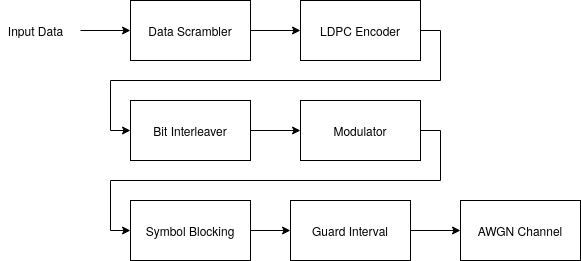
\includegraphics[scale=.5]{phy.png}
\caption{Transmitter block diagram for IEEE802.11ad}
\label{phy}
\end{figure}
\paragraph{} The data scrambler uses a following generator polynomial ($x^7+x^4+1$) to break up the input bitstream. SC-PHY uses low-density parity check codes (LDPC) to perform forward error correction (FEC). The code rates can be any of the following, depending on the choice of modulation scheme: $1/2$, $5/8$, $3/4$, $13/16$, $7/8$. The bits are then passed through an interleaver, and onto a modulator. Modulator can use $\pi/2$-shifted BPSK, QPSK or 16QAM. Then, the data is split into 448-bit blocks, and a 64bit guard interval is placed between. The guard interval consists of a Golay sequence, and modulated with $pi/2$ BPSK. Then, the frame is passed through the AWGN channel, and is then decoded. 
\paragraph{} Performance metrics include bit-error rate curves for the various modulation and coding schemes (MCS) outlined in the specification, and bit rate.


%The specification calls $\pi/2-BPSK$, $\pi/2-QPSK$ and $pi/22-16QAM$ with low density parity check (LDPC) codes of various rates. 


\end{fullwidth}
\end{document}